\section{Durchführung}
\label{sec:Durchführung}

Zuerst wird eine Metallplatte leitend mit zwei Kabeln verbunden, welche die Platte mit dem Konstantstromgerät verbinden. 
Dazu wird ein Multimeter zur Spannungsmessung parallel zur Platte angschlossen und diese wird, wie in Abbildung \ref{fig:Elektromagnet}, auf einer Kunststoffplatte die den Aufbau zusammenhält, zwischen zwei Elektromagneten plaziert.
Mit dem Konstantstromgerät wird ein Querstrom von $I_Q$ angelegt.
Danach wird die magnetische Flussdichte $B$ des Magnetfeldes nach und nach erhöht und die Spannung an der Metallplatte gemessen.
Dies wird für drei Platten durchgeführt, einer aus Kupfer und einer aus Silber, mit $I_Q=\qty{10}{\ampere}$ bei beiden, und ein Draht aus Zink mit $I_Q=\qty{8}{\ampere}$.

Für Kupfer und Silber werden noch die Dicke $d_P$ der Platte gemessen, sowie der Durchmesser der entsprechenden Drähte $d_D$.
Von zwei Spulen die, eine mit Silber und eine mit Kupfer gewickelt sind, wird jeweild der ohmsche Widerstand gemessen.
Die Länge des Drahtes in der Silberspule beträgt $L_S$ und die der Kupferspule $L_K$.

 \begin{figure}[H]
     \centering
     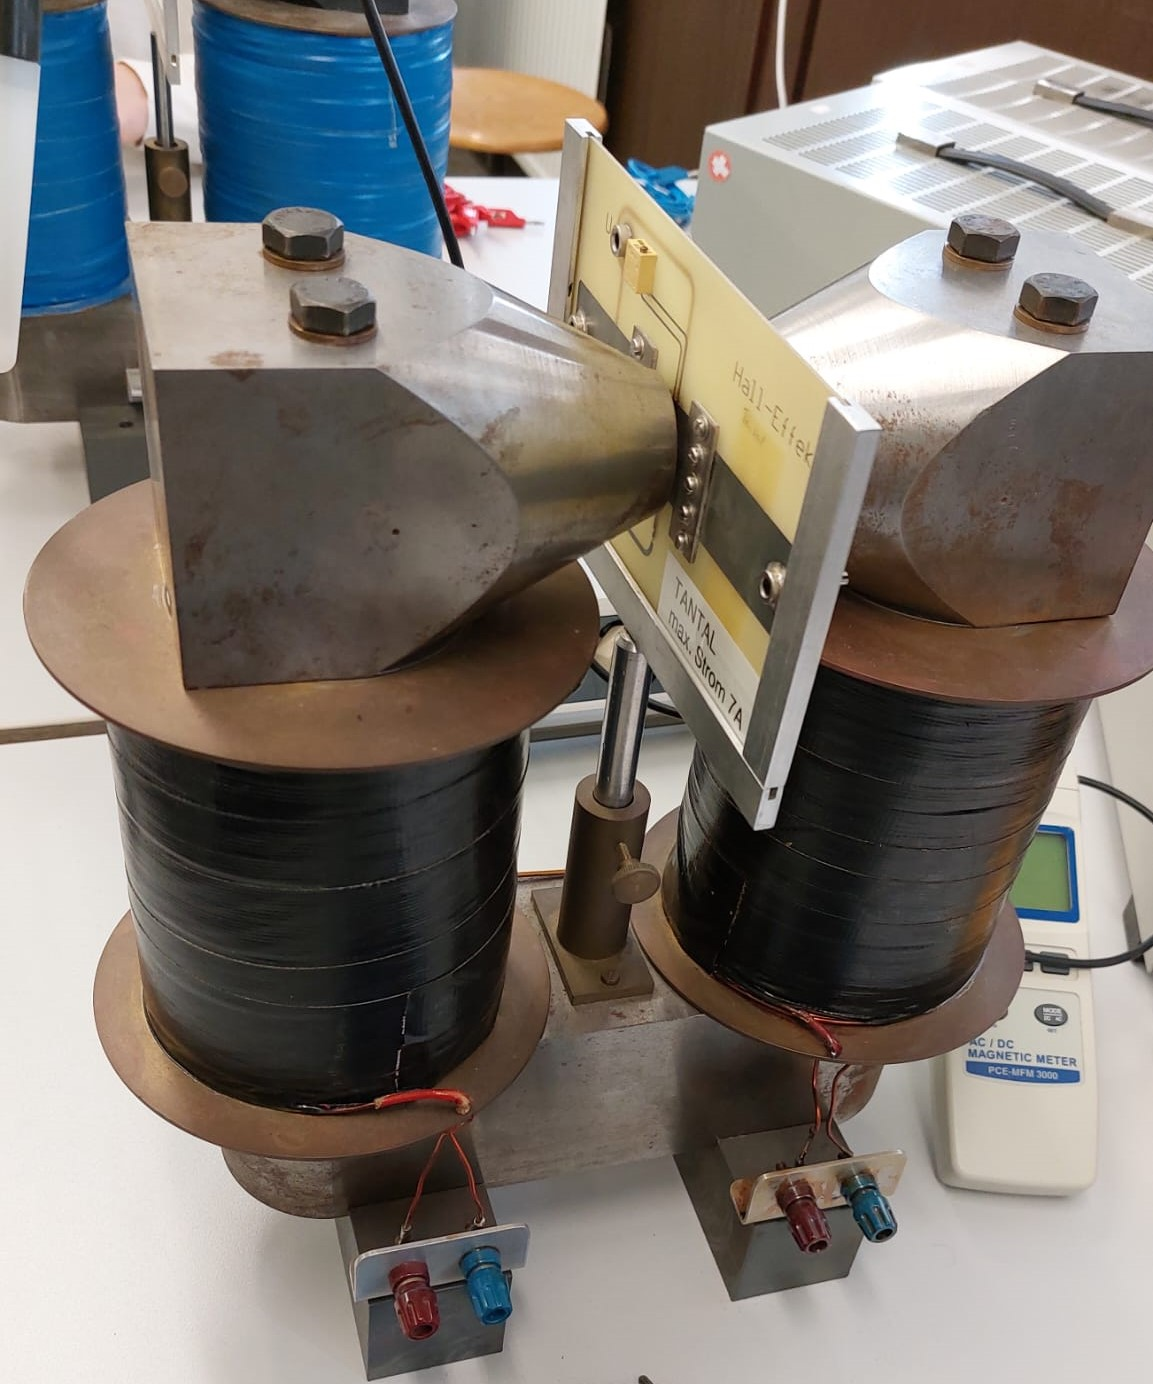
\includegraphics[width=8cm]{Bilder/Elektromagnet.jpg}
     \caption{Abgebildet ist der Aufbau von zwei Elektromagneten mit der Platte dazwischen.}
     \label{fig:Elektromagnet}
 \end{figure}